\documentclass[11pt,letterpaper]{article}
\usepackage[T1]{fontenc}
\usepackage{mathpazo}
\linespread{1.06}
\usepackage[margin=1in,headheight=14pt]{geometry}
\usepackage{amsmath}
\usepackage{microtype}
\usepackage{booktabs}
\usepackage{graphicx}
\usepackage{xcolor}
\usepackage[font=small,labelfont=bf,skip=5pt]{caption}
\usepackage{enumitem}
\usepackage{tcolorbox}
\usepackage{fancyhdr}
\usepackage{lastpage}
\usepackage{titlesec}
\usepackage[hidelinks]{hyperref}

\definecolor{ink}{HTML}{0B0B0B}
\definecolor{muted}{HTML}{52514E}
\definecolor{accent}{HTML}{2A78D6}
\definecolor{boxbg}{HTML}{F3F6FB}

\titleformat{\section}{\large\bfseries\color{ink}}{\thesection}{0.7em}{}
\titlespacing*{\section}{0pt}{1.3\baselineskip}{0.5\baselineskip}
\setlist{itemsep=2pt,topsep=4pt}
\setlength{\parindent}{0pt}
\setlength{\parskip}{5pt}
\renewcommand{\topfraction}{0.9}
\renewcommand{\textfraction}{0.08}
\renewcommand{\floatpagefraction}{0.75}
\setlength{\textfloatsep}{14pt plus 2pt minus 2pt}
\makeatletter\setlength{\@fptop}{0pt}\makeatother
\newcommand{\GeVc}{\,\mathrm{GeV}/c}
% code names in Type 1 Computer Modern typewriter (OT1: no bitmap EC fonts)
\newcommand{\code}[1]{{\fontencoding{OT1}\fontfamily{cmtt}\selectfont #1}}
\newcommand{\pT}{p_T}
\newcommand{\einf}{\varepsilon_\infty}

\pagestyle{fancy}
\fancyhf{}
\renewcommand{\headrulewidth}{0pt}
\fancyfoot[L]{\footnotesize\color{muted}Muon Collider BIB study \,\textperiodcentered\, efficiencies for $p_T\to\infty$}
\fancyfoot[R]{\footnotesize\color{muted}\thepage\ / \pageref{LastPage}}
\fancypagestyle{plain}{\fancyhf{}\fancyfoot[L]{\footnotesize\color{muted}Muon Collider BIB study \,\textperiodcentered\, efficiencies for $p_T\to\infty$}\fancyfoot[R]{\footnotesize\color{muted}\thepage\ / \pageref{LastPage}}}

\begin{document}

{\LARGE\bfseries Signal efficiencies in the limit $\pT\to\infty$\par}
\vspace{4pt}
{\large How the fit of $\einf + c/\pT^2$ to the muons above 10\,GeV/$c$ works\par}
\vspace{6pt}
{\small\color{muted}Muon Collider BIB study \,\textperiodcentered\, 30 September 2026 \,\textperiodcentered\, numbers from run 2026-09-30\_145059\_pdf (the current cuts and resolutions)\par}
\vspace{2pt}
{\color{muted}\rule{\linewidth}{0.4pt}}

\begin{tcolorbox}[colback=boxbg,colframe=boxbg,arc=2pt,left=8pt,right=8pt,top=6pt,bottom=6pt,boxsep=0pt]
The signal hit efficiency and the track-finding efficiency quoted in the results (the summary table and the
highlights PDF) are values in the limit $\pT\to\infty$. Every trial -- a signal hit, or a muon -- with generated
$\pT$ above 10\,GeV/$c$ becomes one data point, at $x = 1/\pT^2$, with $y = 1$ if it passes and $y = 0$ if it
fails. A straight line $y = \einf + c\,x$ is fitted through all these points by least squares, and $\einf$ is
its intercept at $x = 0$, i.e.\ at $\pT\to\infty$. With the current cuts the line comes out flat within its
errors, so $\einf$ is essentially the efficiency of the highest-$\pT$ muons, with an error that does not assume
the flatness.
\end{tcolorbox}

\section{The method, step by step}

\begin{enumerate}[leftmargin=*,label=\textbf{\arabic*.}]
\item \textbf{The trials.} For the signal hit efficiency of a subsystem, each trial is one of the muon's own hits
in that subsystem (hits of its secondaries are left out, \code{muon\_hits\_only = true}). Its outcome is whether
it passes all three cuts of that subsystem -- time, $z_0$ and $\pT$ -- and its $\pT$ is the generated transverse
momentum of the muon that made it, $\pT = \sqrt{p_x^2 + p_y^2}$ from the Monte Carlo truth
(\code{part\_px}, \code{part\_py}; one muon per event). The totals VXD, IT\,+\,OT and ALL pool the hits of
their subsystems. For the track-finding efficiency, each trial is one muon, and its outcome is \emph{found}: at
least 5 of its hits survive the cuts outside the vertex detector.

\item \textbf{The fit range.} Only trials with $\pT > p_{\min}$ enter, where $p_{\min}$ is the larger of
10\,GeV/$c$ and twice the largest $\pT$ cut among the subsystems involved. The largest $\pT$ cut is now
2\,GeV/$c$ (OT only), so $p_{\min} = 10$\,GeV/$c$ everywhere.

\item \textbf{The fit.} With $x_i = 1/p_{T,i}^2$ and $y_i \in \{0, 1\}$, one term per trial in the fit range,
\begin{equation}
S(\einf, c) = \sum_i \bigl(y_i - \einf - c\,x_i\bigr)^2
\end{equation}
is minimized. The minimum follows in closed form from the normal equations,
\begin{equation}
\begin{pmatrix}\einf\\ c\end{pmatrix} = \bigl(X^{\mathsf T}X\bigr)^{-1}X^{\mathsf T}y ,
\qquad X = \begin{pmatrix}1 & x_1\\ \vdots & \vdots\\ 1 & x_n\end{pmatrix},
\end{equation}
so there are no bins, no starting values and no choice other than $p_{\min}$. Since each $y_i$ is 0 or 1, the
line fits the mean efficiency as a function of $x$. A binomial maximum-likelihood fit of the same line gives the
same $\einf$ to within 0.01\,\% (checked for the tracks, the VXD barrel and ALL).

\item \textbf{The uncertainty.} The covariance matrix of $(\einf, c)$ is the ``sandwich'' estimator
\begin{equation}
V = \bigl(X^{\mathsf T}X\bigr)^{-1}\Bigl(\sum_g s_g\, s_g^{\mathsf T}\Bigr)\bigl(X^{\mathsf T}X\bigr)^{-1},
\qquad s_g = \sum_{i\in g} r_i \begin{pmatrix}1\\ x_i\end{pmatrix},
\qquad r_i = y_i - \einf - c\,x_i ,
\end{equation}
and $\sigma(\einf) = \sqrt{V_{11}}$. It is built from the actual scatter of the residuals, so it does not assume
a binomial variance. For the hit efficiencies each group $g$ is one muon: the residuals of its hits are summed
before squaring, because the hits of one muon are not independent. For track-finding each muon is its own group.
In practice the grouping changes little (VXD barrel: 0.093\,\% $\to$ 0.094\,\%;
IT endcap: 0.115\,\% $\to$ 0.122\,\%). A result above 100\,\% would be set to 100\,\%.
\end{enumerate}

{\small\color{muted}\raggedright In the code: \code{efficiency\_at\_infinite\_pt} and \code{pt\_inf\_fit\_min} in
\code{bib\_common.py}, called by \code{apply\_cuts.py} (each subsystem, the VXD, IT\,+\,OT and ALL totals,
and the per-cut tables) and by \code{track\_efficiency.py}.\par}

\section{Why \texorpdfstring{$1/\pT^2$}{1/pT2} and not \texorpdfstring{$1/\pT$}{1/pT}}

Expand the efficiency in the signed curvature $\kappa = q/\pT$ around $\kappa = 0$:
$\varepsilon(\kappa) = \einf + a\,\kappa + b\,\kappa^2 + O(\kappa^3)$. The sample holds as many $\mu^+$ as
$\mu^-$ (50\,145 and 49\,855), so at a given $\pT$ what is measured is the
average over the two charges,
\begin{equation}
\tfrac12\bigl[\varepsilon(\kappa) + \varepsilon(-\kappa)\bigr] = \einf + b\,\kappa^2 + O(\kappa^4)
= \einf + \frac{c}{\pT^2} + \dots
\end{equation}
The linear term cancels exactly, even if the detector responds differently to the two charges. Physically, the
leading effects of a finite momentum all go as $1/p^2$:
\begin{itemize}[leftmargin=1.5em]
\item multiple scattering deflects the muon either way by an rms angle $\propto 1/p$, so the losses it causes go
as its variance, $\propto 1/p^2$;
\item the velocity, $\beta \simeq 1 - m_\mu^2/2p^2$, enters the time of flight;
\item the curvature changes the path length (an arc exceeds its chord by $\simeq s^3/24R^2$) and the
straight-line extrapolation to $z_0$, both by amounts $\propto 1/R^2 \propto 1/\pT^2$.
\end{itemize}
The gun's $\theta$ distribution does not depend on $\pT$, so averaging over $\theta$ turns $1/p^2$ into $c/\pT^2$
with an effective $c$.

\section{\texorpdfstring{Why the fit starts at 10\,GeV/$c$}{Why the fit starts at 10 GeV/c}}

The expansion only holds well above the turn-on of the $\pT$ cut, where the efficiency changes steeply. For OT
barrel hits it is 3.6\,\% at 1.5--2\,GeV/$c$, 85.4\,\% at 2--2.5\,GeV/$c$ and
99.3\,\% at 2.5--3\,GeV/$c$ before it flattens out; the track-finding efficiency has the same
turn-on (Fig.~\ref{fig:tracks}a). Hence the rule: at least twice the largest $\pT$ cut, and never below
10\,GeV/$c$.

\section{Why the extrapolation is short}

The muon gun is flat in $1/\pT$, from $1/1.5$ (GeV/$c$)$^{-1}$ down to almost 0: the highest $\pT$ in the sample
is 120\,TeV/$c$. So 15\,\% of the muons are above 10\,GeV/$c$
(14\,974 of 100\,000), and of those one third are above 30\,GeV/$c$ and one tenth above
100\,GeV/$c$. In $x = 1/\pT^2$ the fit covers $0 < x < 0.01$ (GeV/$c$)$^{-2}$, with a density $\propto x^{-1/2}$:
the points crowd towards $x = 0$ (Fig.~\ref{fig:tracks}b). The intercept is pinned by real data at very high
$\pT$; the slope term only protects it from a bias.

\section{Example: the track-finding efficiency}



The fit gives
\[
\einf = (99.08 \pm 0.11)\,\%, \qquad
c = (0.26 \pm 0.23)\ (\mathrm{GeV}/c)^2 ,
\]
from 14\,974 muons (Table~\ref{tab:tracks}, Fig.~\ref{fig:tracks}).

\begin{figure}[h!]
\centering
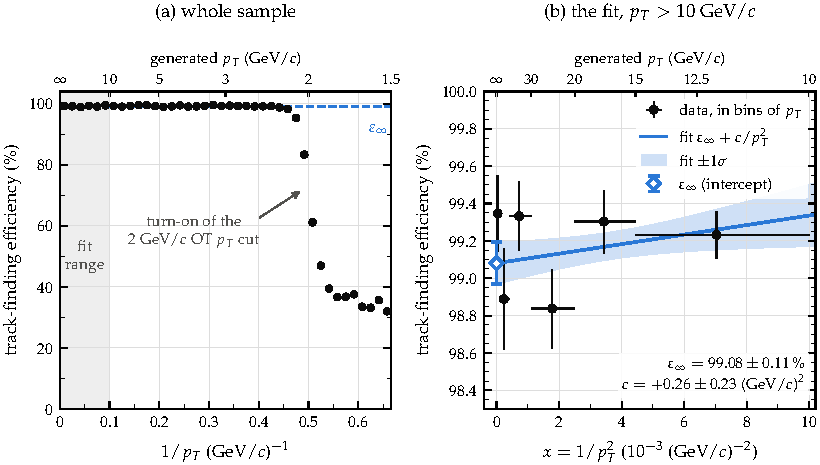
\includegraphics[width=\linewidth]{fig_tracks.pdf}
\caption{Track-finding efficiency (found: at least 5 surviving hits outside the vertex detector).
(a) The whole sample against $1/\pT$, in which the gun is flat, so every bin holds about 2\,500 muons. The
efficiency turns on at the 2\,GeV/$c$ $\pT$ cut of the OT and is flat above it; shaded: the fit range,
$\pT > 10$\,GeV/$c$; dashed: $\einf$. (b) The fit range against $x = 1/\pT^2$ (top axis: $\pT$). The fit uses the
individual muons; the points, in bins of $\pT$ (10--15, 15--20, 20--30, 30--50, 50--100 and above 100\,GeV/$c$,
drawn at their mean $x$, horizontal bars: bin extent), are for display. Line and band: the fitted
$\einf + c/\pT^2$ and its $\pm1\sigma$ band; diamond: $\einf$.}
\label{fig:tracks}
\end{figure}

\begin{table}[t]
\centering
\caption{Track-finding efficiency in bins of generated $\pT$ (display only: the fit uses the individual muons
above 10\,GeV/$c$). Last column: the fitted line at each bin's mean $1/\pT^2$.}
\label{tab:tracks}
\small
\begin{tabular}{l r r r@{\,$\pm$\,}l r}
\toprule
generated $\pT$ (GeV/$c$) & muons & found & \multicolumn{2}{c}{efficiency (\%)} & fit line (\%) \\
\midrule
1.5--2 & 24\,878 & 9\,732 & 39.12 & 0.31 & \multicolumn{1}{c}{--} \\
2--2.5 & 15\,051 & 14\,391 & 95.61 & 0.17 & \multicolumn{1}{c}{--} \\
2.5--5 & 30\,118 & 29\,884 & 99.22 & 0.05 & \multicolumn{1}{c}{--} \\
5--10 & 14\,979 & 14\,873 & 99.29 & 0.07 & \multicolumn{1}{c}{--} \\
\midrule
10--15 & 4\,948 & 4\,910 & 99.23 & 0.12 & 99.26 \\
15--20 & 2\,438 & 2\,421 & 99.30 & 0.17 & 99.17 \\
20--30 & 2\,580 & 2\,550 & 98.84 & 0.21 & 99.13 \\
30--50 & 1\,947 & 1\,934 & 99.33 & 0.18 & 99.10 \\
50--100 & 1\,530 & 1\,513 & 98.89 & 0.27 & 99.09 \\
above 100 & 1\,531 & 1\,521 & 99.35 & 0.21 & 99.08 \\
\midrule
all & 100\,000 & 83\,729 & \multicolumn{2}{l}{83.73} & \\
\bottomrule
\end{tabular}
\end{table}

\begin{itemize}[leftmargin=1.5em]
\item The slope is compatible with zero: above 10\,GeV/$c$ the efficiency is flat within its errors. $\einf$ is
the plain average above 10\,GeV/$c$ (99.17\,\%) minus $c\langle x\rangle$ = 0.08\,\%.
\item Its error is 1.5 times that of the plain average $\bar\varepsilon$. For a straight-line fit
\[
\sigma(\einf) = \sigma(\bar\varepsilon)\,\sqrt{1 + \langle x\rangle^2/\mathrm{Var}(x)} ,
\]
and here $\langle x\rangle = 0.0033$ and $\mathrm{rms}(x) = 0.0030$ (GeV/$c$)$^{-2}$. This is the price of
fitting the slope instead of assuming it is zero.
\item The average over the whole sample, 83.7\,\%, mostly measures how many muons lie below the
2\,GeV/$c$ turn-on. That is why the limit is quoted.
\item Moving the start of the fit changes $\einf$ by at most 0.16\,\%, within its errors:
starting at 5, 7, 10, 15, 20, 40\,GeV/$c$ gives $\einf$ = 99.12, 99.14, 99.08, 99.10, 99.24, 99.21\,\%, with errors from
0.08 to 0.20\,\% (the fits share muons, so these values are not independent).
\end{itemize}



\section{The signal hit efficiencies}

The same fit is made for each subsystem and for the totals (Table~\ref{tab:hits}, Fig.~\ref{fig:hits}). In every
subsystem the slope is compatible with zero within $2\sigma$. Where no $\pT$ cut acts, the hit efficiency is flat
far below 10\,GeV/$c$ as well: in the VXD barrel it is 97.75 $\pm$ 0.05\,\% at
1.5--2\,GeV/$c$ and 97.93 $\pm$ 0.11\,\% at 20--50\,GeV/$c$. That loss is mostly the
Gaussian tail of the 0.03\,ns time smearing outside the $\pm$0.07\,ns cut: $\pm2.3\sigma$ alone gives 98.0\,\%,
and it does not depend on $\pT$. In the OT the whole-sample averages (71--72\,\%) are
again dominated by the turn-on of the 2\,GeV/$c$ cut, while the limits are 99.93\,\% (barrel) and
99.56\,\% (endcap).

\begin{table}[h!]
\centering
\caption{Signal hit efficiency for $\pT\to\infty$: hits and muons in the fit ($\pT > 10$\,GeV/$c$), the fit
results, and, for comparison, the plain averages above 10\,GeV/$c$ and over the whole sample
($\pT \ge 1.5$\,GeV/$c$).}
\label{tab:hits}
\small
\setlength{\tabcolsep}{4.5pt}
\begin{tabular}{l r r r@{\,$\pm$\,}l r@{\,$\pm$\,}l r r}
\toprule
 & & & \multicolumn{2}{c}{$\einf$} & \multicolumn{2}{c}{$c$} & \multicolumn{2}{c}{plain average (\%)} \\
\cmidrule(lr){8-9}
region & hits & muons & \multicolumn{2}{c}{(\%)} & \multicolumn{2}{c}{((GeV/$c$)$^2$)} & $>10$\,GeV/$c$ & all \\
\midrule
VXD barrel & 53\,750 & 13\,440 & 97.80 & 0.09 & $+$0.27 & 0.21 & 97.89 & 97.82 \\
VXD endcap & 19\,720 & 7\,068 & 99.79 & 0.05 & $-$0.11 & 0.13 & 99.76 & 99.83 \\
IT barrel & 24\,920 & 10\,887 & 99.91 & 0.03 & $+$0.05 & 0.06 & 99.92 & 99.89 \\
IT endcap & 40\,022 & 8\,248 & 97.54 & 0.12 & $+$0.44 & 0.26 & 97.69 & 97.18 \\
OT barrel & 19\,670 & 7\,382 & 99.93 & 0.03 & $-$0.11 & 0.08 & 99.89 & 71.43 \\
OT endcap & 23\,789 & 6\,812 & 99.56 & 0.07 & $-$0.22 & 0.16 & 99.48 & 71.89 \\
\midrule
VXD & 73\,470 & 14\,629 & 98.33 & 0.07 & $+$0.19 & 0.15 & 98.39 & 98.35 \\
IT\,+\,OT & 108\,401 & 14\,974 & 98.97 & 0.05 & $+$0.08 & 0.11 & 99.00 & 87.31 \\
ALL & 181\,871 & 14\,974 & 98.71 & 0.04 & $+$0.12 & 0.09 & 98.75 & 91.74 \\
\bottomrule
\end{tabular}
\end{table}

\begin{figure}[t]
\centering
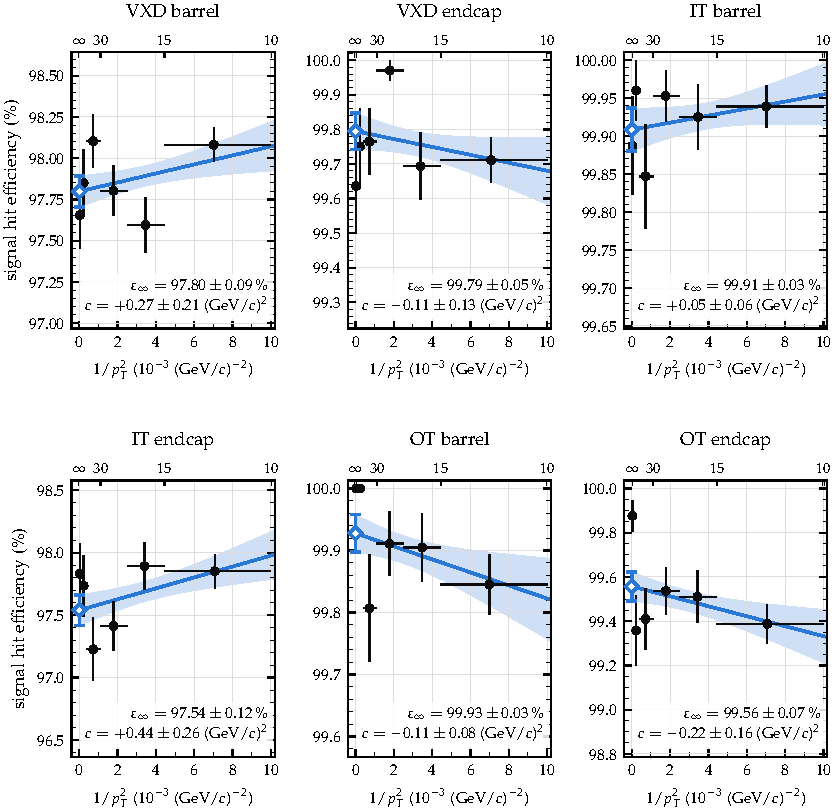
\includegraphics[width=\linewidth]{fig_hits.pdf}
\caption{Signal hit efficiency against $1/\pT^2$ above 10\,GeV/$c$ in the six subsystems, with the fitted line
(symbols as in Fig.~\ref{fig:tracks}b; top axis: $\pT$ in GeV/$c$). The errors of the points are computed per
muon, like those of the fit. Note the different vertical scales.}
\label{fig:hits}
\end{figure}

\end{document}
